
\section{Dasar Git}
\noindent 
 \hspace*{0.5in} Jadi, sebenarnya apa yang dimaksud dengan Git? Ini adalah bagian penting untuk dipahami, karena jika anda memahami apa itu Git dan cara kerja, maka dapat dipastikan anda dapat menggunakan Git secara efektif dengan mudah. Selama menerapkan Git, cobalah untuk menggantikan VCS lain yang mungkin sudah anda kenal sebelumnya, misalnya Subversion dan Perforce. Git sangat berbeda dengan sistem-sistem ini dalam hal simpan atau informasi yang digunakan, meski antar muka sangat mirip. Dengan memahami perbedaan ini diharapkan dapat membantu anda menghindari penggunaan saat menggunakan Git. \par
  \vspace{\baselineskip}
\noindent 
Snapshot, Bukan Perbedaan \par
 \vspace{\baselineskip}
\noindent 
 \hspace*{0.5in} Salah satu perbedaan yang mencolok antar Git dengan VCS lainnya (Subversion dan kawan-kawan) adalah dalam cara Git para datanya. Konsep konseptual,. Sistem seperti ini (CVS, Subversion, Bazaar, dan yang lainnya) informasi yang tersimpannya sebagai sekumpulan berkas dan perubahan yang terjadi pada berkas-berkas tersebut, \par
  \vspace{\baselineskip}
\noindent 
Git dianggap datanya sebagai sebuah kumpulan snapshot dari sebuah miniatur sistem. Setiap kali anda melakukan komit, atau melakukan perubahan pada proyek Git anda, pada butir Git anda secara otomatis. Agar efisien, jika berkas tidak mengalami perubahan, Git tidak akan menyimpan file tersebut pada hanya pada file yang sama yang sebelumnya telah disimpan. \par
 \vspace{\baselineskip}
\noindent 
Git Punya Integritas \par
\noindent 
Segala sesuatu pada Git akan melalui proses checksum terlebih dahulu sebelum disimpan yang kemudian direferensikan oleh hasil checksum tersebut. Hal ini berarti tidak mungkin melakukan perubahan terhadap berkas manapun tanpa diketahui oleh Git.  \par
\noindent 
Fungsionalitas ini dimiliki oleh Git pada level terendahnya dan ini merupakan bagian tak terpisahkan dari filosofi Git. Anda tidak akan kehilangan informasi atau file yang tidak dimiliki oleh Git. \par
 \vspace{\baselineskip}
\noindent 
 \hspace*{0.5in} Mekanisme checksum yang digunakan oleh Git adalah SHA-1 hash. Ini merupakan sebuah susunan string yang terdiri dari 40 karakter heksadesimal (0 sampai 9 dan a sampai f) dan dihitung berdasarkan bentuk dari suatu berkas atau struktur pada pada Git. sebuah hash SHA-1 seperti berikut: \par
\noindent 
Anda akan melihat seperti ini pada berbagai tempat di Git. Faktanya, Git tidak memiliki nama file pada basisdatanya, pela nilai hash dari isi berkas. \par
\noindent 
Secara Umum Git Hanya Selesai Data \par
 \vspace{\baselineskip}
\noindent 
Bila anda melakukan operasi pada Git, hanya dari penambahan data pada basisdata Git. Sangat sulit membuat sistem melakukan sesuatu yang tidak bisa diurungkan atau membuatnya menghapus data dengan cara apa pun.  \par
 \vspace{\baselineskip}
\noindent 
Seperti pada berbagai VCS, anda bisa kehilangan atau mengacaukan perubahan yang belum di-commit; namun jika anda melakukan komit pada Git, akan sangat sulit kehilanngannya, apalagi jika anda secara teratur melakukan push basisdata anda pada repositori lain. Hal ini membuat Git menyenangkan karena kita dapat berexperimen tanpa kehawatiran untuk mengacaukan proyek. Untuk lebih jelas dan dalam lagi tentang bagaimana Git menyimpan datanya dan bagaimana anda bisa mengembalikan yang hilang \par
 \vspace{\baselineskip}
\noindent 
Direktori Git adalah dimana Git menyimpan metadata dan database objek untuk projek anda. Ini adalah bahagian penting dari Git, dan inilah yang disalin saat anda melakukan kloning sebuah repositori dari komputer lain. \par
\noindent 
Direktori kerja adalah sebuah checkout tunggal dari satu versi dari projek. File-berkas ini kemudian ditarik keluar dari basisdata yang terkompresi dalam direktori Git dan disimpan pada disk untuk anda pakai atau modifikasi. \par
\noindent 
 \hspace*{0.5in} Alur kerja dasar Git adalah seperti ini: \par
\noindent 
 \hspace*{0.5in} Anda mengubah berkas dalam direktori kerja anda. \par
\noindent 
 \hspace*{0.5in} Anda membawa ke tahap, menambahkan snapshotnya ke area stage. \par
\noindent 
 \hspace*{0.5in} Anda melakukan komit  \par
  \vspace{\baselineskip}
\noindent 
Jika sebuah versi tertentu dari sebuah berkas telah ada di direktori git, ia dianggap 'berkomitmen'. Jika berkas diubah (sudah diubah) maka sudah ditambahkan ke area stage, maka itu adalah 'staged'. Dan jika berkas telah diubah sejak terakhir dilakukan check out belum ditambahkan ke area stage maka itu adalah 'modified'. \par
\noindent 
Pada, anda akan lebih banyak membahas mengenai keadaan-keadaan ini dan bagaimana anda dapat memanfaatkan keadaan-keadaan yang bersangkutan dengan bagian 'bertahap'. \par
 \vspace{\baselineskip}
\noindent 
Git adalah $  $\textit{version control system} $  $yang digunakan para developer untuk mengembangkan software secara bersama-bersama. Fungsi utama git yaitu mengatur versi dari source code program anda dengan mengasih tanda baris dan code mana yang ditambah atau diganti.  Git ini sebenernya memudahkan programmer untuk mengetahui perubahan source codenya daripada harus membuat file baru seperti $  $\textit{Program.java, ProgramRevisi.java,}\textit{ }\textit{ProgramRevisi2.java, ProgramFix.java}. Selain itu, dengan git kita tak perlu khawatir code yang kita kerjakan bentrok, karena setiap developer bias membuat branch sebagai $  $\textit{workspace}nya.Fitur yang tak kalah keren lagi, pada git kita bisa memberi komentar pada source code yang telah ditambah/diubah, hal ini mempermudah developer lain untuk tahu $  $ kendala apa yang dialami developer lain. \par
 \vspace{\baselineskip}
\noindent 
Untuk mengetahui bagaimana menggunakan git, berikut perintah-perintah dasar git: \par
\noindent 
\begin{enumerate}
\item Git init : untuk membuat $  $\textit{repository} $  $pada file lokal yang nantinya ada folder .git \par
\noindent 
\item Git status : untuk mengetahui status dari $  $\textit{repository} $  $lokal \par
\noindent 
\item Git add : menambahkan file baru pada $  $\textit{repository} $  $yang dipilih \par
\noindent 
\item Git commit : untuk menyimpan perubahan yang dilakukan, tetapi tidak ada perubahan pada $  $\textit{remote repository.} \par
\noindent 
\item Git push : untuk mengirimkan perubahan file setelah di commit ke $  $\textit{remote repository.} \par
\noindent 
\item Git branch : melihat seluruh $  $\textit{branch $  $}yang ada pada repository \par
\noindent 
\item Git checkout : menukar $  $\textit{branch $  $}yang aktif dengan $  $\textit{branch}yang dipilih \par
\noindent 
\item GIt merge : untuk menggabungkan $  $\textit{branch $  $}yang aktif dan $  $\textit{branch $  $}yang dipilih \par
\noindent 
\item Git clone : membuat Salinan $  $\textit{repository $  $}lokal\end{enumerate}
 \par
 
  \begin{itemize}
 	\item The Many (Faces) Stages Of Git
 \end{itemize}
 
  \begin{figure}[ht]
 	\centerline{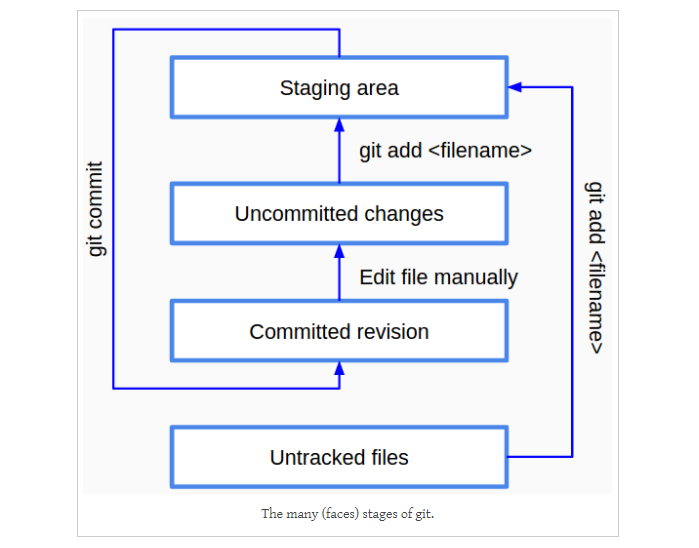
\includegraphics[width=0.70\textwidth]{figures/GitReview}}
 	\caption{Stages Of Git}
 	\label{Satges Of Git}
 \end{figure}
 
 \vspace{\baselineskip}
\noindent 
Contoh dari $  $\textit{software version control system} $  $adalah github, bitbucket, snowy evening, dan masih banyak lagi. Jika anda sebagai developer belum mengetahui fitur git ini, maka anda wajib mencoba dan memakainya. Karena banyak manfaat yang akan didapat dengan git ini. \par
\noindent 
Git itu bukanlah sebuah bahasa seperti halnya HTML,CSS atau Js bukan pula sebuah konsep atau aturan baku dalam pemrograman, melainkan sebuah software yang berfungsi untuk mengatur source code dari aplikasi yang sedang anda buat. \par
\vspace{12pt}
\noindent 
Fungsi utamanya adalah untuk mengatur versi dari source code anda, menambahkan tanda/checkpoint ketika terjadi perubahan pada kode Anda dan tentunya akan mempermudah Anda untuk tetap mengetahui apa saja yang berubah dari source code Anda. \par
\noindent 
Sebagai contoh, misalkan Anda sedang membangun sebuah website, dan anda akan menambahkan beberapa fitur dalam website anda. Agar tidak membingungkan nantinya anda membuat sebuah catatan terhadap apa yang telah anda lakukan seperti : \par
\noindent 
 \hspace*{0.5in} 01-04-2014 Memulai Project Website, File HTML  $  \&  $ CSS Dasar \par
\noindent 
 \hspace*{0.5in} 02-04-2014 Penambahan Menu Utama \par
\noindent 
 \hspace*{0.5in} 03-04-2014 Penambahan Layout Standar \par
\noindent 
 \hspace*{0.5in} 04-04-2014 Penambahan Fitur Pengubah Layout \par
\vspace{\baselineskip}
\noindent 
Pada contoh diatas kita menggunakan tanggal sebagai tanda akan apa yang telah kita lakukan, dengan demikian kita bisa tahu kapan perubahan terjadi dan apa perubahan yang dilakukan.  \par
\vspace{\baselineskip}
\noindent 
Dan dalam Git semua itu bisa dilakukan dengan mudah dan asyiknya jika Anda merusak kode sehingga membuat aplikasi error, maka anda dapat mengembalikan kode tersebut berdasarkan pada tanda/tanggal dimana kode masih normal, lebih mirip seperti restore point. \par
\vspace{\baselineskip}
\noindent 
Git juga tidak hanya digunakan untuk perorangan, beberapa orang pun dapat bekerja secara bersamaan mengerjakan kode Anda dan Anda masih memiliki kontrol penuh terhadap kode Anda,  \par
\vspace{\baselineskip}
\noindent 
Anda bisa menambahkan kode yang ditambahan oleh orang lain atau mengabaikannya sama sekali. oleh karena itu Git sering digunakan sebagai pengatur dalam projek kolaborasi dimana tidak hanya satu orang yang mengerjakan sebuah kode tapi beberapa orang sekaligus yang mengerjakan kode tersebut. \par
\vspace{\baselineskip}
\noindent 
Misalkan anda ingin menambahkan suatu fitur, namun anda tidak mau kode yang ada sekarang rusak karena fitur yang akan anda tambahkan masih belum stabil,  \par
\vspace{\baselineskip}
\noindent 
Dalam Git anda dapat membuat branch terlebih dahulu. Branch ini bisa diartikan sebagai cabang dari branch master. segala perubahan yang anda lakukan pada branch yang anda buat tidak akan berpengaruh pada branch lainnya. \par
\vspace{\baselineskip}
\noindent 
Sebagai contoh, kita buat branch dengan nama branch  $ " $fix-css $ " $ dengan mengetikkan perintah: \par
\noindent 
 \hspace*{0.5in} git branch fix-css \par
\noindent 
Jika perintah dijalankan dengan benar maka ketika anda mengetikkan perintah git branch akan muncul branch-branch yang telah dibuat. \par
\noindent 
 \hspace*{0.5in} ~~ fix-css \par
\noindent 
 \hspace*{0.5in} *~~ master \par
\noindent 
tanda Bintang menandakan bahwa anda sedang bekerja pada branch master, untuk berpindah ke branch yang baru saja dibuat (fix-css) ketikkan perintah berikut: \par
\noindent 
 \hspace*{0.5in} git checkout fix-css \par
\noindent 
Jika peritah di atas benar, maka akan ada pemberitahuan seperti berikut: \par
\noindent 
 \hspace*{0.5in} Switched to branch 'fix-css' \par
\noindent 
Github  \par
\noindent 
Github merupakan situs sharing code dan menggunakan git sebagai SCM-nya. Mungkin Anda pernah mendownload beberapa library/source code dari situs ini. Kini anda tahu mengapa kebanyakan source code dapat anda temui di github. \par
\vspace{12pt}
\noindent 
\subsection{Apa itu GIT?} 
\noindent 
Git adalah version control, dengan menggunakan Git kita dapat menyimpan tiap perubahan yang kita lakukan pada file. Seperti menggunakan  $ " $undo $ " $ tetapi dapat digunakan pada seluruh file kita dan kita mempunyai log pada tiap perubahan yang kita simpan, Hal ini sangat berguna pada production environment, karena dengan adanya versioning, kita dapat dengan mudah melakukan rollback. Selain itu Git juga sangat membantu dalam proses pengembangan aplikasi. Salah satu platform Git yang terkenal adalah GitHub. Kita akan menggunakan GitHub untuk artiketl berikut. \par
\vspace{12pt}
\noindent 
\section{Repository}
\noindent 
Di Git Repository biasanya digunakan untuk mengorganisir sebuah projek. Projek dapat berisi files, folder, gambar, video dan lainnya yang dibutuhkan untuk sebuah project. Kami menyarankan untuk menambahkan file README yang bertujuan untuk memberi informasi terkait isi dari project tersebut. Kita dapat mengasumsikan Repository sebagai folder untuk menyimpan project kita. Satu berada di Local, dan yang satu berada di Remote disini kita menggunakan GitHub. \par
\vspace{12pt}
\vspace{12pt}

{\fontsize{14pt}{14pt}\selectfont \textbf{Seperti Ini Review}\textbf{ Changes} \\} \par
\vspace{\baselineskip}
\noindent 
Setelah melihat rincian komit, Jerry menyadari bahwa panjang string tidak boleh negatif, karena itulah dia memutuskan untuk mengubah jenis fungsi my $  \_  $strlen yang kembali. \par
\vspace{\baselineskip}
\noindent 
Jerry menggunakan perintah git log untuk melihat detail log. \par
\vspace{\baselineskip}
\noindent 
\begin{verbatim}
  $ git log 
\end{verbatim}
\noindent 

\begin{verbatim}
 Perintah di atas akan menghasilkan hasil berikut.
 melakukan cbe1249b140dad24b2c35b15cc7e26a6f02d2277 
 Penulis: Jerry Mouse <jerry@tutorialspoint.com>
 Tanggal: Rabu Sep 11 08:05:26 2013 +0530 
 Diimplementasikan fungsi my_strlen
 \end{verbatim}
 
 \vspace{\baselineskip}
\noindent 
Jerry menggunakan perintah git show untuk melihat rincian komit. Perintah git show mengambil SHA-1 commit ID sebagai parameter. \par
\vspace{\baselineskip}
\noindent 
\begin{verbatim}
$ git show cbe1249b140dad24b2c35b15cc7e26a6f02d2277 
Perintah di atas akan menghasilkan hasil sebagai berikut: 
melakukan cbe1249b140dad24b2c35b15cc7e26a6f02d2277 
Penulis: Jerry Mouse <jerry@tutorialspoint.com> 
Tanggal: Rabu Sep 11 08:05:26 2013 +0530 
Diimplementasikan fungsi my_$strlen 
 \end{verbatim}
 
 \vspace{\baselineskip}
 \vspace{12pt}
\noindent 
 \hspace*{0.5in} diff - git a / string.c b / string.c \par
\noindent 
 \hspace*{0.5in} mode file baru 100644 \par
\noindent 
 \hspace*{0.5in} indeks 0000000..187afb9 \par
\noindent 
 \hspace*{0.5in} --- / dev / null \par
\noindent 
 \hspace*{0.5in} +++ b / string.c \par
\noindent 
 \hspace*{0.5in} @@ -0,0 +1,24 @@ \par
\noindent 
 \hspace*{0.5in} +  $  \#  $ include <stdio.h> \par
\noindent 
 \hspace*{0.5in} + \par
\noindent 
 \hspace*{0.5in} + int my $  \_  $strlen (char * s) \par
\noindent 
 \hspace*{0.5in} +  $  \{  $ \par
\noindent 
 \hspace*{0.5in}  $  $ $  $ $  $+ \par
\noindent 
 \hspace*{0.5in}  $  $ $  $ $  $char * p = s; \par
\noindent 
 \hspace*{0.5in}  $  $ $  $ $  $+ \par
\noindent 
 \hspace*{0.5in}  $  $ $  $ $  $+ \par
\noindent 
 \hspace*{0.5in}  $  $ $  $ $  $sementara (* p) \par
\noindent 
 \hspace*{0.5in}  $  $ $  $ $  $+ ++ p; \par
\noindent 
 \hspace*{0.5in}  $  $ $  $ $  $+ return (p -s); \par
\noindent 
 \hspace*{0.5in}  $  $ $  $ $  $+ \par
\noindent 
 \hspace*{0.5in}  $  \}  $ \par
\noindent 
 \hspace*{0.5in} + \par
 \vspace{\baselineskip}
\noindent 
Dia mengubah jenis fungsi kembali dari int menjadi size $  \_  $t. Setelah menguji kode tersebut, dia mengulas perubahannya dengan menjalankan perintah diff git. \par
\vspace{\baselineskip}
\noindent 
 \hspace*{0.5in}  $  \$  $ git diff \par
\noindent 
Perintah di atas akan menghasilkan hasil sebagai berikut: \par
\noindent 
 \hspace*{0.5in} diff - git a / string.c b / string.c \par
\noindent 
 \hspace*{0.5in} indeks 187afb9..7da2992 100644 \par
\noindent 
 \hspace*{0.5in} --- a / string.c \par
\noindent 
 \hspace*{0.5in} +++ b / string.c \par
\noindent 
 \hspace*{0.5in} @@ -1,6 +1,6 @@ \par
\noindent 
 \hspace*{0.5in}  $  \#  $include <stdio.h> \par
\noindent 
 \hspace*{0.5in} -int my $  \_  $strlen (char * s) \par
\noindent 
 \hspace*{0.5in} + size $  \_  $t my $  \_  $strlen (char * s) \par
\noindent 
 \hspace*{0.5in}  $  \{  $ \par
\noindent 
 \hspace*{0.5in}  $  $ $  $ $  $char * p = s; \par
\noindent 
 \hspace*{0.5in}  $  $ $  $ $  $@@ -18,7 +18,7 @@ int main (void) \par
\noindent 
 \hspace*{0.5in}  $  \}  $; \par
\noindent 
 \hspace*{0.5in} untuk (i = 0; i <2; ++ i) \par
\noindent 
 \hspace*{0.5in}  $  \{  $ \par
\noindent 
 \hspace*{0.5in}  $  $ $  $ $  $- printf ("panjang string $  \%  $ s = $  \%  $ d  $  \setminus  $ n", s [i], my $  \_  $strlen (s [i])); \par
\noindent 
 \hspace*{0.5in}  $  $ $  $ $  $+ printf ("panjang string $  \%  $ s = $  \%  $ lu  $  \setminus  $ n", s [i], my $  \_  $strlen (s [i])); \par
\noindent 
 \hspace*{0.5in}  $  $ $  $ $  $kembali 0; \par
\noindent 
 \hspace*{0.5in}  $  \}  $ \par
 \vspace{\baselineskip}
\noindent 
Git diff menunjukkan tanda '+' sebelum baris, yang baru ditambahkan dan '-' untuk baris yang dihapus. \par
\noindent 
Melihat Sejarah Komit \par
\vspace{\baselineskip}
\noindent 
 \hspace*{0.5in} Setelah Anda membuat beberapa commit, atau jika Anda telah mengkloning sebuah repositori dengan riwayat komit yang ada, Anda mungkin ingin melihat kembali untuk melihat apa yang telah terjadi. Alat yang paling dasar dan ampuh untuk melakukan ini adalah perintah git log. \par
 \vspace{\baselineskip}
\noindent 
Contoh-contoh ini menggunakan proyek sederhana yang disebut "simplegit". Untuk mendapatkan proyek, jalankan \par
\noindent 
git klon https://github.com/schacon/simplegit-progit \par
\noindent 
Saat Anda menjalankan git log dalam proyek ini, Anda harus mendapatkan keluaran yang terlihat seperti ini: \par
\noindent 
 \hspace*{0.5in}  $  \$  $ git log \par
\noindent 
 \hspace*{0.5in} melakukan ca82a6dff817ec66f44342007202690a93763949 \par
\noindent 
 \hspace*{0.5in} Penulis: Scott Chacon <schacon@gee-mail.com> \par
\noindent 
 \hspace*{0.5in} Tanggal: Sen 17 Mar 21:52:11 2008 -0700 \par
\noindent 
 \hspace*{0.5in}  $  $ $  $ $  $ $  $mengubah nomor versinya \par
\noindent 
 \hspace*{0.5in} komit 085bb3bcb608e1e8451d4b2432f8ecbe6306e7e7 \par
\noindent 
 \hspace*{0.5in} Penulis: Scott Chacon <schacon@gee-mail.com> \par
\noindent 
 \hspace*{0.5in} Tanggal: Sat 15 Mar 16:40:33 2008 -0700 \par
\noindent 
lepaskan tes yang tidak perlu \par
\noindent 
 \hspace*{0.5in} lakukan a11bef06a3f659402fe7563abf99ad00de2209e6 \par
\noindent 
 \hspace*{0.5in} Penulis: Scott Chacon <schacon@gee-mail.com> \par
\noindent 
 \hspace*{0.5in} Tanggal: Sat Mar 15 10:31:28 2008 -0700 \par
\noindent 
 $  $ $  $ $  $ $  $komit pertama \par
 \vspace{\baselineskip}
\noindent 
Secara default, tanpa argumen, git log mencantumkan komit yang dibuat di repositori tersebut dalam urutan kronologis terbalik - yaitu, komit terbaru muncul lebih dulu. Seperti yang dapat Anda lihat, perintah ini mencantumkan masing-masing komit dengan checksum SHA-1, nama penulis dan e-mail, tanggal penulisan, dan pesan komit. \par
\noindent 
Sejumlah besar dan berbagai pilihan untuk perintah git log tersedia untuk menunjukkan dengan tepat apa yang Anda cari. Di sini, kami akan menunjukkan beberapa yang paling populer. \par
\vspace{\baselineskip}
\noindent 
Salah satu pilihan yang lebih bermanfaat adalah -p, yang menunjukkan perbedaan yang diperkenalkan pada masing-masing komit. Anda juga bisa menggunakan -2, yang membatasi output hanya pada dua entri terakhir: \par

\noindent 
 \hspace*{0.5in}  $  \$  $ git log -p -2 \par
\noindent 
 \hspace*{0.5in} melakukan ca82a6dff817ec66f44342007202690a93763949 \par
\noindent 
 \hspace*{0.5in} Penulis: Scott Chacon <schacon@gee-mail.com> \par
\noindent 
 \hspace*{0.5in} Tanggal: Sen 17 Mar 21:52:11 2008 -0700 \par
\noindent 
 \hspace*{0.5in}  $  $ $  $ $  $ $  $mengubah nomor versinya \par
\noindent 
 \hspace*{0.5in} diff - git a / Rakefile b / Rakefile \par
\noindent 
 \hspace*{0.5in} indeks a874b73..8f94139 100644 \par
\noindent 
 \hspace*{0.5in} --- a / Rakefile \par
\noindent 
 \hspace*{0.5in} +++ b / Rakefile \par
\noindent 
 \hspace*{0.5in} @@ -5,7 +5,7 @@ memerlukan 'rake / gempackagetask' \par
\noindent 
 \hspace*{0.5in}  $  $spec = Gem :: Specification.new do  $  \vert  $ s  $  \vert  $ \par
\noindent 
 \hspace*{0.5in}  $  $ $  $ $  $ $  $ $  $s.platform = Gem :: Platform :: RUBY \par
\noindent 
 \hspace*{0.5in}  $  $ $  $ $  $ $  $ $  $s.name = "simplegit" \par
\noindent 
 \hspace*{0.5in} - s.version = "0.1.0" \par
\noindent 
 \hspace*{0.5in} + s.version = "0.1.1" \par
\noindent 
 \hspace*{0.5in}  $  $ $  $ $  $ $  $ $  $s.author = "Scott Chacon" \par
\noindent 
 \hspace*{0.5in}  $  $ $  $ $  $ $  $ $  $s.email = "schacon@gee-mail.com" \par
\noindent 
 \hspace*{0.5in}  $  $ $  $ $  $ $  $ $  $s.summary = "Sebuah permata sederhana untuk menggunakan Git dalam kode Ruby." \par
\noindent 
 \hspace*{0.5in} komit 085bb3bcb608e1e8451d4b2432f8ecbe6306e7e7 \par
\noindent 
 \hspace*{0.5in} Penulis: Scott Chacon <schacon@gee-mail.com> \par
\noindent 
 \hspace*{0.5in} Tanggal: Sat 15 Mar 16:40:33 2008 -0700 \par
\noindent 
 \hspace*{0.5in}  $  $ $  $ $  $ $  $lepaskan tes yang tidak perlu \par
\noindent 
 \hspace*{0.5in}  \hspace*{0.5in} diff - git a / lib / simplegit.rb b / lib / simplegit.rb \par
\noindent 
 \hspace*{0.5in}  \hspace*{0.5in} indeks a0a60ae..47c6340 100644 \par
\noindent 
 \hspace*{0.5in}  \hspace*{0.5in} --- a / lib / simplegit.rb \par
\noindent 
 \hspace*{0.5in}  \hspace*{0.5in} +++ b / lib / simplegit.rb \par
\noindent 
 \hspace*{0.5in}  \hspace*{0.5in} @@ -18,8 +18,3 @@ kelas SimpleGit \par
\noindent 
 \hspace*{0.5in}  \hspace*{0.5in}  $  $ $  $ $  $ $  $ $  $akhir \par
\noindent 
 \hspace*{0.5in}  $  $akhir \par
\noindent 
 \hspace*{0.5in} - \par
\noindent 
 \hspace*{0.5in} -if  $  \$  $ 0 ==  $  \_  $ $  \_  $FILE $  \_  $ $  \_  $ \par
\noindent 
 \hspace*{0.5in} - git = SimpleGit.new \par
\noindent 
 \hspace*{0.5in} - menempatkan git.show \par
\noindent 
 \hspace*{0.5in} -akhir \par
\noindent 
 \hspace*{0.5in}  $  \setminus  $ Tidak ada baris baru di akhir file \par
 \vspace{\baselineskip}
\noindent 
 \hspace*{0.5in} Pilihan ini menampilkan informasi yang sama namun dengan diff langsung mengikuti setiap entri. Ini sangat membantu untuk tinjauan kode atau untuk menelusuri dengan cepat apa yang terjadi selama serangkaian komit yang telah ditambahkan oleh kolaborator. Anda juga bisa menggunakan serangkaian opsi merangkum dengan log git. Misalnya, jika Anda ingin melihat beberapa statistik singkat untuk setiap komit, Anda dapat menggunakan opsi --stat: \par
 \vspace{\baselineskip}
\noindent 
 \hspace*{0.5in}  $  \$  $ git log --stat \par
\noindent 
 \hspace*{0.5in} melakukan ca82a6dff817ec66f44342007202690a93763949 \par
\noindent 
 \hspace*{0.5in} Penulis: Scott Chacon <schacon@gee-mail.com> \par
\noindent 
 \hspace*{0.5in} Tanggal: Sen 17 Mar 21:52:11 2008 -0700 \par
 \vspace{\baselineskip}
\noindent 
 \hspace*{0.5in}  $  $ $  $ $  $ $  $mengubah nomor versinya \par
\noindent 
 \hspace*{0.5in}  $  $Rakefile  $  \vert  $ 2 + - \par
\noindent 
 \hspace*{0.5in}  $  $1 file berubah, 1 insertion (+), 1 deletion (-) \par
\noindent 
 \hspace*{0.5in} komit 085bb3bcb608e1e8451d4b2432f8ecbe6306e7e7 \par
\noindent 
 \hspace*{0.5in} Penulis: Scott Chacon <schacon@gee-mail.com> \par
\noindent 
 \hspace*{0.5in} Tanggal: Sat 15 Mar 16:40:33 2008 -0700 \par
 \vspace{\baselineskip}
\noindent 
 \hspace*{0.5in}  $  $ $  $ $  $ $  $lepaskan tes yang tidak perlu \par
\noindent 
 \hspace*{0.5in}  $  $lib / simplegit.rb  $  \vert  $ 5 ----- \par
\noindent 
 \hspace*{0.5in}  $  $1 file berubah, 5 deletions (-) \par
 \vspace{\baselineskip}
\noindent 
 \hspace*{0.5in} lakukan a11bef06a3f659402fe7563abf99ad00de2209e6 \par
\noindent 
 \hspace*{0.5in} Penulis: Scott Chacon <schacon@gee-mail.com> \par
\noindent 
 \hspace*{0.5in} Tanggal: Sat Mar 15 10:31:28 2008 -0700 \par
 \vspace{\baselineskip}
\noindent 
 \hspace*{0.5in}  $  $ $  $ $  $ $  $komit pertama \par
\noindent 
 $  $ \hspace*{0.5in}  \hspace*{0.5in} README  $  \vert  $ 6 ++++++ \par
\noindent 
 \hspace*{0.5in}  $  $ \hspace*{0.5in} Rakefile  $  \vert  $ 23 +++++++++++++++++++++++ \par
\noindent 
 $  $ \hspace*{0.5in}  \hspace*{0.5in} lib / simplegit.rb  $  \vert  $ 25 +++++++++++++++++++++++++ \par
\noindent 
 \hspace*{0.5in}  \hspace*{0.5in}  $  $3 file berubah, 54 sisipan (+) \par

